\section{Classification}

Observe that the classification procedures for multivariate data described in
Section~\ref{sec:multivariate_classification} (the maximum depth classifier,
the DD classifier, and the DD$^G$ classifier) only depend on the data through
the depth feature vectors
\begin{equation}
    \vx^D = (D(\vx, F_1), \dots, D(\vx, F_k)) \in \R^k.
\end{equation}
By simply choosing an appropriate functional data depth $D$, all of these
classification procedures naturally generalize to the functional setting.
The most flexible of these is the DD$^G$ classifier
\parencite{albertos-bande-fuente-2017}, which allows for any multivariate
classification procedure on the transformed data $\mathscr{D}^D$.



\begin{figure}
    \centering
    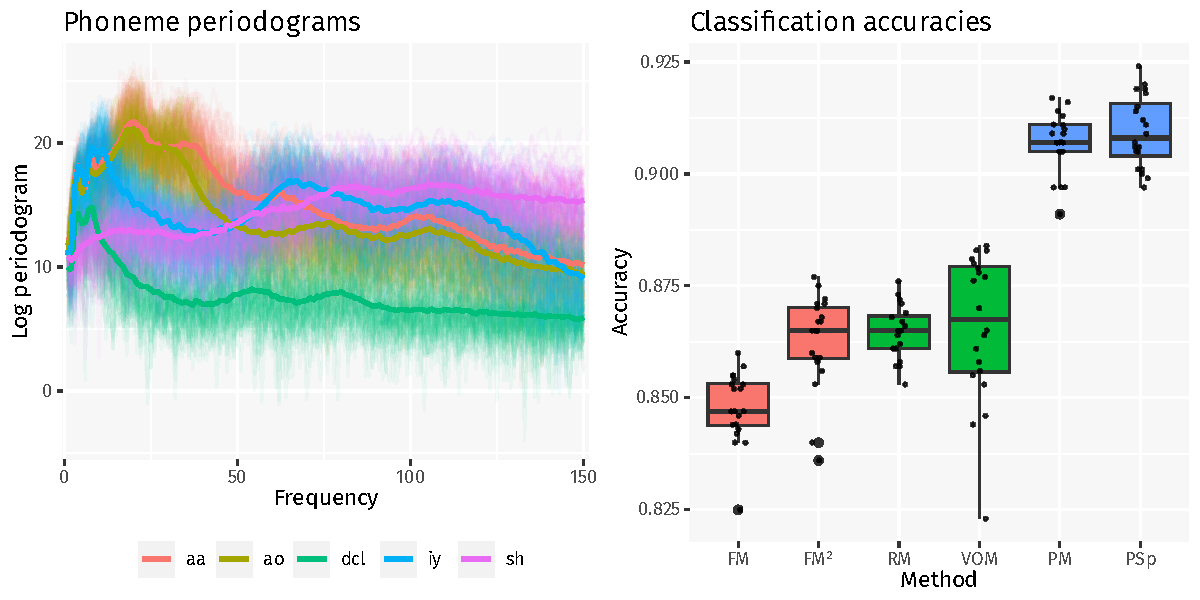
\includegraphics[width = \textwidth, page = 1]{phoneme}
    \caption{
        Classification of periodograms of digitized
        speech\protect\footnotemark, by phonemes (`aa', `ao', `dcl', `iy',
        `sh').
        The thick colored lines in the plot on the left mark the median curve
        across 400 examples in each of the five groups.
        The boxplot shows classification accuracies for 20 runs of each of the
        following methods: maximum depth classification using the first order
        (FM) and second order (FM$^2$) Fraiman-Muniz depths in red, the RM and
        VOM classifiers in green, and the maximum depth Mahalanobis (PM) and
        spatial (PSp) depth classifiers on $d$-variate feature vectors
        obtained by $d = 10$ random projections in blue.
        In each run, 50\% of the data was been aside for training.
    }
    \label{fig:phoneme_classification}
\end{figure}
\footnotetext{\url{http://www-stat.stanford.edu/ElemStatLearn}}



\subsection{Outlyingness matrices}

\textcite{dai-genton-2018} proposed a method which measures the outlyingness
of $\vx$ with respect to a population via depth as follows.

\begin{definition}
    Let $\vX$ be a $d$-variate stochastic process of continuous functions.
    At each time point $t \in [0, 1]$, the directional outlyingness is defined
    as
    \begin{equation}
        \vO(t) = \vO(\vX(t), F_{\vX(t)}) = \left(\frac{1}{D(\vX(t), F_{\vX(t)})} - 1\right)\, \vv(t),
    \end{equation}
    where $\vv(t)$ is the unit vector pointing from the median of $F_{\vX(t)}$
    to $\vX(t)$.
\end{definition}

\begin{definition}
    The functional directional outlyingness is defined as
    \begin{equation}
        \FO(\vX, F_{\vX}) = \int_{[0, 1]} \norm{\vO(t)}^2 \:w(t)\:dt.
    \end{equation}
\end{definition}

\begin{definition}
    \label{def:MO}
    The mean directional outlyingness is defined as
    \begin{equation}
        \MO(\vX, F_{\vX}) = \int_{[0, 1]} \vO(t) \:w(t)\:dt.
    \end{equation}
\end{definition}

\begin{definition}
    The variation of directional outlyingness is defined as
    \begin{equation}
        \VO(\vX, F_{\vX}) = \int_{[0, 1]} \norm{\vO(t) - \MO(t)}^2 \:w(t)\:dt.
    \end{equation}
\end{definition}

Here, $w$ is a weight function on $[0, 1]$.
In our discussion, we set $w = 1$.

It is easily verified that
\begin{equation}
    \FO^2 = \norm{\MO}^2 + \VO.
\end{equation}

\textcite{dai-genton-2018} propose using the $(d + 1)$-variate feature vectors
\begin{equation}
    \vY(\vX, F_{\vX}) = (\MO^\top,\, \VO)^\top
\end{equation}
corresponding to the curve $\vX$ for the purposes of classification.
The $\MO$ gives a sense of how outlying the curve $\vX$ is within $F_{\vX}$ as
a whole, while the $\VO$ measures the amount of variation in the outlyingness
over time.
Loosely speaking, $\MO$ is affected by the position, while $\VO$ is affected
by the shape of $\vX$ within $F_{\vX}$.
For instance, one may define the classifier
\begin{equation}
    \hat{\iota}(\vX) = \argmax_{1 \leq i \leq k} D'(\vY(\vX, F_i), F_{\vY(\vX, F_i)}),
\end{equation}
where $D'$ is a multivariate depth function.
This is simply a maximum depth classifier applied on the feature vectors
$\vY$.
When $D'$ is chosen to be the robust Mahalanobis depth, we have the RM
classifier
\begin{equation}
    \hat{\iota}_{RM}(\vX) = \argmax_{1 \leq i \leq k} D_{RM}(\vY(\vX, F_i), F_{\vY(\vX, F_i)}).
\end{equation}


\begin{definition}
    The functional directional outlyingness matrix is defined as
    \begin{equation}
        \FOM(\vX, F_{\vX}) = \int_{[0, 1]} \vO(t)\,\vO(t)^\top \:w(t)\:dt.
    \end{equation}
\end{definition}

\begin{definition}
    The functional directional outlyingness matrix is defined as
    \begin{equation}
        \VOM(\vX, F_{\vX}) = \int_{[0, 1]} (\vO(t) - \MO(t))\,(\vO(t) - \MO(t))^\top \:w(t)\:dt.
    \end{equation}
\end{definition}

Again, it is easily verified that
\begin{equation}
    \FOM = \MO\,\MO^\top + \VOM,
\end{equation}
and that
\begin{equation}
    \FO = \tr(\FOM), \qquad
    \VO = \tr(\VOM).
\end{equation}

We may also use the feature matrix $\VOM$, or its matrix norm $\norm{\VOM}_F$
corresponding to the curve $\vX$ for the purposes of classification.
Here, $\norm{\Cdot}_F$ denotes the Frobenius norm.
For instance, a $\VOM$ based classifier may be defined as
\begin{equation}
    \hat{\iota}_{\VOM}(\vX) = \argmin_{1 \leq i \leq k} \norm{\VOM(\vX, F_i)}_F.
\end{equation}



\subsection{Random projections}

Another approach is to use a feature vector consisting of multiple projections
of $\vX$.
Given functions $\vv_1, \dots, \vv_d$ chosen at random, we examine the
$d$-variate feature vectors
\begin{equation}
    \bm{V}(\vX, F_{\vX}) = \left(\ip{\vv_1}{\vX}, \dots, \ip{\vv_d}{\vX}\right)
\end{equation}
and apply a depth based multivariate classifier.
For instance, given a multivariate depth function $D'$, we may define a
classifier
\begin{equation}
    \hat{\iota}^d_{D'}(\vX) = \argmax_{1 \leq i \leq k} D'(\bm{V}(\vX, F_i), F_{\bm{V}(\vX, F_i)}).
\end{equation}
